\documentclass[12pt,a4paper]{report}

% Packages required
\usepackage[utf8]{inputenc}
\usepackage[top=1in, bottom=1in, left=1.25in, right=1in]{geometry}
\usepackage{graphicx}
\usepackage{booktabs}
\usepackage{tabularx}
\usepackage{pifont}
\usepackage{pgfgantt}
\usepackage[edges]{forest}
\usepackage{tikz}
\usepackage{hyperref}
\usepackage{setspace}
\usepackage{titlesec}
\usepackage{xcolor}
\usepackage{fancyhdr}
\usepackage{tikz}
\usetikzlibrary{positioning, shapes.geometric, arrows.meta}
\definecolor{wbsRoot}{RGB}{0, 80, 80}       % Dark Teal
\definecolor{wbsPhase}{RGB}{95, 158, 160}   % Medium Teal
\definecolor{wbsTask}{RGB}{215, 235, 235}   % Light Mint

% Footer setup to match the PDF
\pagestyle{fancy}
\fancyhf{}
\fancyfoot[C]{\thepage}
\renewcommand{\headrulewidth}{0pt}
\fancyfoot[L]{\footnotesize Capital University of Science and Technology, Islamabad}
\fancyfoot[R]{\footnotesize Department of Computer Science}
\renewcommand{\footrulewidth}{0.4pt}

% Customizing chapter heading format
\titleformat{\chapter}[display]
  {\normalfont\huge\bfseries}{\chaptertitlename\ \thechapter}{20pt}{\Huge}
\titlespacing*{\chapter}{0pt}{-20pt}{40pt}

% Define checkmark and cross
\newcommand{\cmark}{\ding{51}}
\newcommand{\xmark}{\ding{55}}

\setstretch{1.4}

\begin{document}

% ==========================================
% TITLE PAGE
% ==========================================
\begin{titlepage}
\thispagestyle{empty}
    \begin{center}
        \vspace*{0.6cm}

        {\LARGE \bfseries Mazdoor Link \\[0.3cm]
       
        \par}

        \vspace{1.2cm}

        \begin{tabular}{lcl}
            \large BILAL AZIZ & \large : & \large BCS231019\\[0.25cm]
            \large HANZALA HABIB AWAN & \large : & \large BCSP251011\\[0.25cm]
            \large MUHAMMAD WASIF RAFIQ & \large : & \large BCSP251006
        \end{tabular}

        \vspace{1.2cm}

        % University Logo - place logo.jpg in same folder as your .tex file
        
\includegraphics[width=0.28\textwidth]{log.jpg}

        \vspace{1.0cm}

        {\large \bfseries Supervised By}\\[0.2cm]
        {\large Ms.\ Rabea Saleem}\\[0.8cm]

        {\large \bfseries Spring-2026}\\[0.8cm]

        {\large \bfseries Department of Computer Science}\\[0.2cm]
        {\large \bfseries Capital University of Science \& Technology, Islamabad}

    \end{center}
\end{titlepage}

% ==========================================
% FRONT MATTER
% ==========================================
\pagenumbering{arabic}
\setcounter{page}{1}

\tableofcontents
\newpage
\listoftables
\newpage
\listoffigures
\newpage

% ==========================================
% CHAPTER 1
% ==========================================
\chapter{Introduction}

This chapter provides a brief summary of the project scope, project specification, a comparison study with the available existing solutions, and existing tools and technologies that may be used for the development of this project. This chapter also includes a project work breakdown structure and a proposed timeline.

\section{Project Introduction}

In the current socio-economic landscape of Pakistan, a significant portion of the urban population regularly requires skilled labor services such as plumbing, electrical work, carpentry, painting, and general home maintenance. Despite the high demand for these services, the process of finding and hiring reliable workers remains largely informal, unstructured, and inefficient. Customers typically rely on personal references, local contacts, or random phone numbers obtained through word-of-mouth, which often leads to a lack of trust, no price transparency, poor communication, and an overall unsatisfactory service experience \cite{ilo}.

At the same time, skilled workers in Pakistan face significant challenges in securing consistent job opportunities. The majority of these workers belong to low-literacy demographics with limited digital access and minimal exposure to technology-based platforms. Existing methods of job acquisition, such as standing at designated labor gathering points (\textit{labour chowks}) or relying on intermediaries, are inherently inefficient and do not guarantee regular employment. This dual-sided problem creates a substantial communication and accessibility gap between customers seeking services and workers offering them \cite{pbs}.

The proposed system, titled \textbf{MazdoorLink AI} (alternatively \textbf{UstaadConnect}), aims to address these challenges by providing a comprehensive, AI-powered smart labor hiring and communication platform designed specifically for the Pakistani market. The platform is delivered as a unified cross-platform mobile application that supports three distinct user roles: Customer, Worker, and Administrator.

The core workflow of the proposed system is as follows. A customer initiates the process by either searching for a specific type of worker, selecting from pre-defined job templates for common tasks, or posting a custom job request describing the required service. Customers can also schedule bookings for future dates and times, allowing for better planning of home maintenance tasks. The system's AI-powered job matching engine then identifies and recommends the most suitable workers based on multiple parameters including skill category, geographic proximity, real-time availability, and historical ratings. The customer can review worker profiles, which include verified credentials, past job ratings, service photos from previous work, and available service packages, before confirming the booking. Customers can also save frequently used workers to their favorites list for quick access in future bookings.

A critical innovation of the proposed system is its focus on bridging the technology gap for non-technical workers. Recognizing that a large proportion of Pakistani laborers have limited literacy and are not technology-friendly, the system incorporates voice-based interaction capabilities. Workers can speak instead of typing, with speech-to-text technology converting their voice input into system-processable data. The interface is designed primarily in Urdu, the national language, with simplified one-tap buttons for key actions such as toggling online/offline availability, accepting or rejecting jobs, and viewing earnings. Automatic location detection eliminates the need for manual address entry, and optional call-based interaction is supported for workers who prefer traditional communication methods \cite{ahmed2021}.

Furthermore, the system integrates a smart chat translation feature that enables seamless English-to-Urdu and Urdu-to-English communication between customers and workers, effectively eliminating the language barrier that frequently hinders service coordination. The platform includes an integrated time tracking system that automatically monitors work duration, providing transparency for both customers and workers regarding service time. Workers can create service packages offering bundled services at discounted rates, such as combined plumbing and electrical work, enabling them to increase their earning potential.

To ensure safety and trust, the platform incorporates a comprehensive labor verification process. Workers are required to submit their CNIC (Computerized National Identity Card) with front and back images, a police clearance certificate, and pay a refundable security deposit that serves as financial assurance against potential damages or disputes. The security deposit is held by the platform and returned to workers at the end of each month, provided no verified damage claims have been filed against them. Only workers who successfully pass the verification process and pay the security deposit are listed on the platform, providing customers with the assurance that they are hiring vetted and trustworthy individuals. Additionally, workers must complete OTP (One-Time Password) verification during registration to ensure phone number authenticity.

The main actors of the proposed system include the Customer, Worker, and Administrator, all of whom access the system through the same mobile application with role-specific interfaces. The Customer can search for services using smart filters, post jobs manually or select from quick-access job templates, book workers for immediate or scheduled future service, save preferred workers to a favorites list, track service progress in real-time with GPS-based location tracking, monitor work duration through the integrated time tracker, communicate via chat or voice with automatic translation, view before-and-after service photos, make secure in-app payments, and provide ratings and reviews. In case of service issues or property damage, customers can submit detailed damage reports with photographic evidence through the platform's dedicated reporting system.

The Worker can register with simplified onboarding that includes CNIC and police clearance document upload, pay a refundable monthly security deposit, complete OTP verification, manage availability status with a single-tap toggle, receive instant push notifications for nearby job opportunities, view scheduled bookings in a calendar interface, accept or reject job requests, interact with the system through voice commands for hands-free operation, create and manage service packages for bundled offerings, upload before-and-after photos of completed work to build a portfolio, use the integrated time tracker to record actual work hours, communicate with customers via auto-translated chat, navigate to job locations using integrated GPS, track daily, weekly, and monthly earnings through a visual dashboard, and view their ratings and customer reviews.

The Administrator manages the overall platform through a dedicated admin interface within the mobile application, including user account management, worker verification by reviewing submitted CNIC and police clearance documents, processing and approving security deposit payments, handling damage reports by reviewing evidence from both parties and making fair decisions, dispute resolution between customers and workers, managing the security deposit refund process at month-end, viewing platform analytics including total users, active jobs, and revenue statistics, configuring service categories and platform settings such as commission rates, and monitoring system health and user feedback.

The proposed system is developed as a cross-platform mobile application using Flutter for deployment on both Android and iOS platforms, Firebase services including Authentication for OTP-based user login, Firestore for real-time NoSQL cloud database, Cloud Storage for storing images and documents, and Cloud Messaging for push notifications. The backend business logic is implemented using Firebase Cloud Functions with Node.js, and Python-based AI modules are deployed as separate microservices for natural language processing, speech recognition, machine learning-based job matching, and smart chat translation. This technology stack ensures scalability, security, real-time synchronization, and cross-platform accessibility, enabling all stakeholders to access the system through their Android or iOS mobile devices.

\section{Existing Examples / Solutions}

There are a number of applications and platforms currently operating in or relevant to the Pakistani labor hiring market that provide services for connecting customers with skilled workers. In the following section, some of these existing solutions are listed and compared with the proposed system.

\subsection{Karsaaz App}
Karsaaz is a Pakistani mobile application that connects customers with home service providers including plumbers, electricians, painters, and other skilled workers. Launched as a marketplace for blue-collar services, Karsaaz allows customers to browse service categories, view worker profiles, and book services through the app. The platform provides basic worker registration and customer review functionality. However, Karsaaz does not incorporate any AI-powered features such as intelligent job matching, voice-based interaction for low-literacy workers, smart chat translation, or scheduled booking capabilities. The platform's interface is primarily in English, creating a significant usability barrier for Urdu-speaking workers with limited literacy. Additionally, it lacks advanced features such as service packages, time tracking, damage reporting mechanisms, and worker security deposits \cite{karsaaz}.

\subsection{Kam Kaaj}
Kam Kaaj is a Lahore-based home services platform that offers a range of domestic services including cleaning, plumbing, electrical work, and handyman services. The platform operates through a mobile application and website, allowing customers to book verified service providers. Kam Kaaj emphasizes service quality through a vetting process for workers. However, the platform does not provide AI-based job matching, voice-based worker interaction, real-time bilingual chat translation, scheduled bookings, job templates for quick posting, or worker-created service packages. Additionally, the platform's digital interface is not specifically designed for low-literacy users, and it does not support voice-based navigation, Urdu-first interface design, or comprehensive damage liability management through security deposits \cite{kamkaaj}.

\subsection{HomeServices.pk}
HomeServices.pk is a Pakistani web-based platform that provides a directory of home service providers across multiple cities in Pakistan. The platform enables customers to search for workers by service category and location, and provides basic contact information for service providers. While the platform serves as a useful directory, it lacks a transactional booking system, real-time tracking, in-app communication, AI-powered features, scheduled booking functionality, favorites management, worker verification mechanisms, time tracking, damage reporting, and mobile application support. The platform functions primarily as a listing service without the intelligent matching and communication capabilities proposed in the current system \cite{homeservices}.

\subsection{TaskBid (International Reference)}
TaskBid is an international task-based hiring platform that allows customers to post tasks and receive bids from available workers. The platform incorporates a bidding mechanism where workers compete for jobs, and includes features such as worker profiles, ratings, and in-app messaging. TaskBid demonstrates a viable business model with commission-based revenue generation. However, the platform is not designed for the Pakistani market, does not support Urdu language, does not incorporate voice-based interaction for low-literacy users, and does not include AI-powered features such as intelligent job matching based on local context, speech-to-text functionality, smart chat translation, scheduled bookings, job templates, service packages, time tracking, or damage liability management through security deposits \cite{taskbid}.

Table \ref{tab:comparison} presents a comparison of features between the existing solutions and the proposed MazdoorLink AI platform.

\begin{table}[h]
    \centering
    \caption{Existing Solutions Features Comparison}
    \label{tab:comparison}
    \vspace{0.2cm}
    \resizebox{\textwidth}{!}{
    \begin{tabular}{clccccc}
        \toprule
        \textbf{Sr.} & \textbf{Characteristics} & \textbf{Karsaaz} & \textbf{Kam Kaaj} & \textbf{HomeServices} & \textbf{TaskBid} & \textbf{MazdoorLink AI}\\
        & & \textbf{App} & & \textbf{.pk} & & \textbf{(Proposed)}\\
        \midrule
        1 & Worker Registration & \cmark & \cmark & \xmark & \cmark & \cmark \\
        2 & OTP Verification & \cmark & \xmark & \xmark & \cmark & \cmark \\
        3 & AI Job Matching & \xmark & \xmark & \xmark & \xmark & \cmark \\
        4 & Voice-Based Interaction & \xmark & \xmark & \xmark & \xmark & \cmark \\
        5 & Urdu Language Support & \xmark & \xmark & \xmark & \xmark & \cmark \\
        6 & Smart Chat Translation & \xmark & \xmark & \xmark & \xmark & \cmark \\
        7 & Scheduled Bookings & \xmark & \cmark & \xmark & \xmark & \cmark \\
        8 & Favorite Workers & \xmark & \xmark & \xmark & \xmark & \cmark \\
        9 & Job Templates & \xmark & \xmark & \xmark & \xmark & \cmark \\
        10 & Service Packages & \xmark & \xmark & \xmark & \xmark & \cmark \\
        11 & Time Tracker & \xmark & \xmark & \xmark & \xmark & \cmark \\
        12 & Service Photos & \xmark & \cmark & \xmark & \xmark & \cmark \\
        13 & Worker Verification & \xmark & \cmark & \xmark & \xmark & \cmark \\
        14 & Damage Reporting & \xmark & \xmark & \xmark & \xmark & \cmark \\
        15 & Security Deposit & \xmark & \xmark & \xmark & \xmark & \cmark \\
        16 & Real-Time GPS Tracking & \xmark & \xmark & \xmark & \xmark & \cmark \\
        17 & Rating \& Review & \cmark & \cmark & \xmark & \cmark & \cmark \\
        18 & In-App Communication & \cmark & \xmark & \xmark & \cmark & \cmark \\
        19 & Low-Literacy UI Design & \xmark & \xmark & \xmark & \xmark & \cmark \\
        20 & Cross-Platform Mobile App & \cmark & \cmark & \xmark & \cmark & \cmark \\
        21 & Police Clearance Check & \xmark & \xmark & \xmark & \xmark & \cmark \\
        \bottomrule
    \end{tabular}
    }
\end{table}

As evident from Table \ref{tab:comparison}, the proposed MazdoorLink AI platform offers a unique combination of features that are not collectively available in any single existing solution in the Pakistani market. While platforms like Karsaaz and Kam Kaaj provide basic service booking capabilities, none of the existing solutions offer the comprehensive feature set including AI-powered job matching, voice-based interaction for low-literacy workers, smart bilingual chat translation, scheduled bookings, job templates for quick posting, favorite workers management, service packages, integrated time tracking, before-and-after service photos, comprehensive damage reporting with security deposit protection, and worker verification including police clearance checks. The proposed system fills this critical gap by providing an intelligent, inclusive, and trust-oriented platform specifically designed for Pakistan's informal labor market.

\section{Business Scope}

The informal labor sector in Pakistan constitutes a significant portion of the national economy, with an estimated 40 million workers engaged in skilled and semi-skilled trades including plumbing, electrical work, carpentry, painting, masonry, and general home maintenance services \cite{pbs}. Despite the massive scale of this workforce, the sector remains largely undigitized, with service discovery, hiring, and payment conducted through informal channels that lack transparency, accountability, and efficiency.

The proposed MazdoorLink AI platform targets the rapidly growing urban centers of Pakistan, including Islamabad, Karachi, Lahore, Rawalpindi, and Faisalabad, where the demand for skilled labor services is consistently high. The system addresses critical pain points experienced by both customers and workers, including the difficulty of finding reliable workers, the absence of price standardization, communication barriers between English-speaking customers and Urdu-speaking workers, lack of worker verification mechanisms, absence of damage liability protection, and the inability of low-literacy workers to utilize existing technology platforms.

The platform has strong business potential through multiple revenue streams. The primary revenue model is a commission-based structure, where the platform charges a 5--15\% service fee on each completed job transaction. Additional revenue can be generated through featured worker listings, where workers pay a premium to appear at the top of search results; subscription plans for workers seeking enhanced visibility and priority job notifications; one-time or monthly security deposit processing fees; and advertisement placements by related businesses such as hardware stores, tool suppliers, and construction material providers.

The adoption of such a platform can lead to significant improvements in service quality, customer satisfaction, and worker income stability. Studies on gig economy platforms in developing countries have reported increases of up to 35\% in worker earnings and a 45\% improvement in customer satisfaction when digital intermediation is introduced into informal labor markets \cite{worldbank}.

Furthermore, the AI-powered features of the proposed system, including intelligent job matching, voice-based interaction, and real-time chat translation, provide a competitive advantage over existing platforms that rely solely on manual search and basic listing functionalities. The cloud-based architecture utilizing Firebase services ensures that the system can be deployed with minimal infrastructure, reducing the total cost of deployment and enabling rapid scaling to new cities and regions.

The comprehensive safety and liability management system, including mandatory security deposits, damage reporting workflows, and worker verification, addresses a critical gap in existing platforms and provides significant value to customers who are concerned about trusting unknown workers in their homes. This feature alone can serve as a major differentiator and adoption driver in the Pakistani market.

The system also presents opportunities for collaboration with government initiatives such as the Punjab Information Technology Board (PITB) and the Ehsaas Program, which aim to digitize public services and provide economic support to marginalized communities. By providing a verified database of skilled workers with digital records, the platform can serve as a valuable resource for government workforce development and skills certification programs. The initial deployment is planned for Islamabad, with subsequent expansion to other major cities based on user adoption and market demand.

\subsection{Safety and Liability Management}

One of the most significant concerns in the informal labor market is the risk of property damage or disputes during service provision. To address this critical issue, the proposed platform implements a comprehensive multi-layered protection mechanism that ensures accountability and provides recourse for both customers and workers.

Workers are required to pay a refundable security deposit ranging from PKR 5,000 to PKR 10,000 upon successful registration and verification. This deposit serves as financial assurance against potential damages or service-related disputes. The security deposit is held securely by the platform and is fully refundable at the end of each month, provided that no verified damage claims have been filed against the worker during that period. This monthly refund cycle ensures that workers maintain good standing continuously and provides an ongoing incentive for professional conduct.

The damage reporting system allows customers to submit detailed incident reports with photographic evidence directly through the mobile application. When a damage report is filed, the platform administrator is immediately notified and initiates a review process. The administrator contacts both the customer and the worker to gather statements and evidence from both parties. Both customers and workers are strongly encouraged to take before-and-after photographs of the work site at the beginning and completion of each job, creating a transparent and timestamped record that can be referenced objectively in case of disputes.

If a damage claim is verified by the administrator after reviewing evidence from both sides, the appropriate compensation amount is deducted from the worker's security deposit and transferred to the customer. The worker's rating is also reduced, and the incident is recorded in their profile. Workers who accumulate multiple verified damage reports face progressive penalties including further rating reductions, temporary suspension, and potential permanent removal from the platform if the pattern of problematic behavior continues.

This system creates a balanced approach that protects customers from financial loss due to negligent or malicious damage while also protecting workers from false or exaggerated claims through the administrator-mediated review process. The transparency provided by timestamped photographs and the financial stake represented by the security deposit work together to create a trust-based ecosystem that encourages professional service delivery and honest reporting.

\section{Useful Tools and Technologies}

The following tools and technologies are selected for the development of the proposed MazdoorLink AI platform. The selection is based on factors including performance, scalability, cross-platform compatibility, AI integration capabilities, real-time synchronization, community support, cost-effectiveness, and alignment with industry best practices.

\subsection{Mobile Frontend: Flutter}
Flutter is an open-source UI software development kit created by Google for building natively compiled applications for mobile, web, and desktop from a single codebase. Flutter uses the Dart programming language and provides a rich set of pre-designed widgets that enable the creation of visually appealing and highly responsive user interfaces. Flutter's hot reload feature significantly accelerates the development cycle by allowing developers to see changes in real-time without restarting the application.

Flutter is selected as the mobile frontend framework for the proposed system due to its ability to produce a single codebase that runs on both Android and iOS platforms, which is essential for maximizing user reach in the Pakistani market where both operating systems are prevalent. Flutter's widget-based architecture is well-suited for implementing the simplified, low-literacy-friendly interface required for the worker-side application, including large one-tap buttons, voice input integration, and Urdu text rendering. The framework's excellent performance characteristics ensure smooth animations and responsive interactions even on lower-end devices commonly used by the target worker demographic.

\subsection{Backend: Firebase Services}
Firebase is a comprehensive mobile and web application development platform provided by Google that offers a suite of cloud-based services including authentication, real-time database, cloud storage, cloud functions, and push notifications. Firebase provides automatic scaling, built-in security, real-time data synchronization, and seamless integration with Flutter applications.

Firebase is selected as the primary backend infrastructure for the proposed system due to several compelling advantages. \textbf{Firebase Authentication} provides secure OTP-based phone number verification, which is essential for ensuring user authenticity without requiring email addresses that many workers may not have. \textbf{Cloud Firestore} is a flexible, scalable NoSQL cloud database that stores data in JSON-like documents, allowing for dynamic schemas that can evolve with application requirements. Firestore's real-time synchronization capabilities are essential for live features such as instant job notifications, real-time chat messaging, and GPS location tracking updates.

\textbf{Firebase Cloud Storage} provides secure, scalable object storage for user-uploaded content including CNIC images, police clearance certificates, before-and-after service photos, and user profile pictures. The storage service integrates seamlessly with Firebase Security Rules to ensure that only authorized users can access sensitive documents.

\textbf{Firebase Cloud Functions} allows the deployment of backend business logic as serverless functions written in Node.js. These functions can be triggered by database events, HTTP requests, or scheduled tasks, enabling complex workflows such as automatic notification sending, commission calculation, monthly security deposit refunds, and integration with external AI services.

\textbf{Firebase Cloud Messaging (FCM)} provides reliable, battery-efficient push notification delivery to both Android and iOS devices, ensuring that workers receive instant job alerts and customers receive booking confirmations and status updates.

The cloud-hosted nature of Firebase eliminates the need for on-premises server infrastructure, reduces operational complexity, and provides automatic scaling to handle varying loads as the platform grows.

\subsection{AI and Machine Learning: Python}
Python is a high-level, general-purpose programming language widely recognized as the leading language for artificial intelligence, machine learning, and natural language processing applications. Python's extensive ecosystem of AI libraries, including TensorFlow, PyTorch, scikit-learn, NLTK, and spaCy, provides comprehensive tools for developing intelligent systems.

Python is selected for implementing the AI-powered core features of the proposed system, including the intelligent job matching algorithm using machine learning-based recommendation models that consider worker skills, location proximity, availability, historical ratings, and customer preferences. The speech-to-text module for voice-based worker interaction utilizes the Google Cloud Speech-to-Text API with Urdu language support, enabling workers to interact naturally without typing. The smart chat translation engine for English-Urdu bilingual communication is implemented using the Google Cloud Translation API with neural machine translation models, ensuring contextually accurate translations that preserve meaning across languages.

These Python-based AI services are deployed as separate microservices that expose REST APIs, which are consumed by Firebase Cloud Functions to integrate AI capabilities seamlessly into the mobile application workflow.

\subsection{Speech and Translation APIs}
The proposed system integrates specialized APIs for speech recognition and language translation to enable voice-based interaction and bilingual communication.

\textbf{Google Cloud Speech-to-Text API} is used to convert worker voice input into text, supporting Urdu language recognition. This API provides high-accuracy speech recognition with support for multiple languages and dialects, enabling workers to interact with the system through natural speech instead of typing \cite{google_speech}.

\textbf{Google Cloud Translation API} is used to provide real-time English-to-Urdu and Urdu-to-English translation within the chat module, enabling seamless communication between customers and workers who may prefer different languages \cite{google_translation}.

\subsection{Development Tools}
\begin{itemize}
    \item \textbf{Visual Studio Code:} A lightweight, extensible source code editor developed by Microsoft, used for Flutter and Node.js development with rich plugin support for Dart, Firebase, and Git integration.
    \item \textbf{Android Studio:} The official IDE for Android development, used for Flutter mobile application testing and debugging with Android emulators and physical device testing.
    \item \textbf{Firebase Console:} The web-based administration interface for Firebase services, used for monitoring database activity, managing authentication, viewing analytics, and configuring security rules.
    \item \textbf{Git \& GitHub:} A distributed version control system and a cloud-based repository hosting service, used for source code management, version tracking, and team collaboration.
    \item \textbf{Postman:} An API development and testing tool, used for testing the backend RESTful APIs and Firebase Cloud Functions during development.
\end{itemize}

\section{Project Work Break Down}

The project is divided into five major phases: Requirements Gathering, Requirement Analysis, Design, Implementation, and Testing. The work breakdown structure in Figure \ref{fig:wbs} illustrates the decomposition of the project into manageable tasks and the assignment of responsibilities to each team member.
% ==========================================
% WORK BREAKDOWN STRUCTURE DIAGRAM
% ==========================================
\begin{figure}[!htbp]
    \centering
    \resizebox{\textwidth}{!}{
    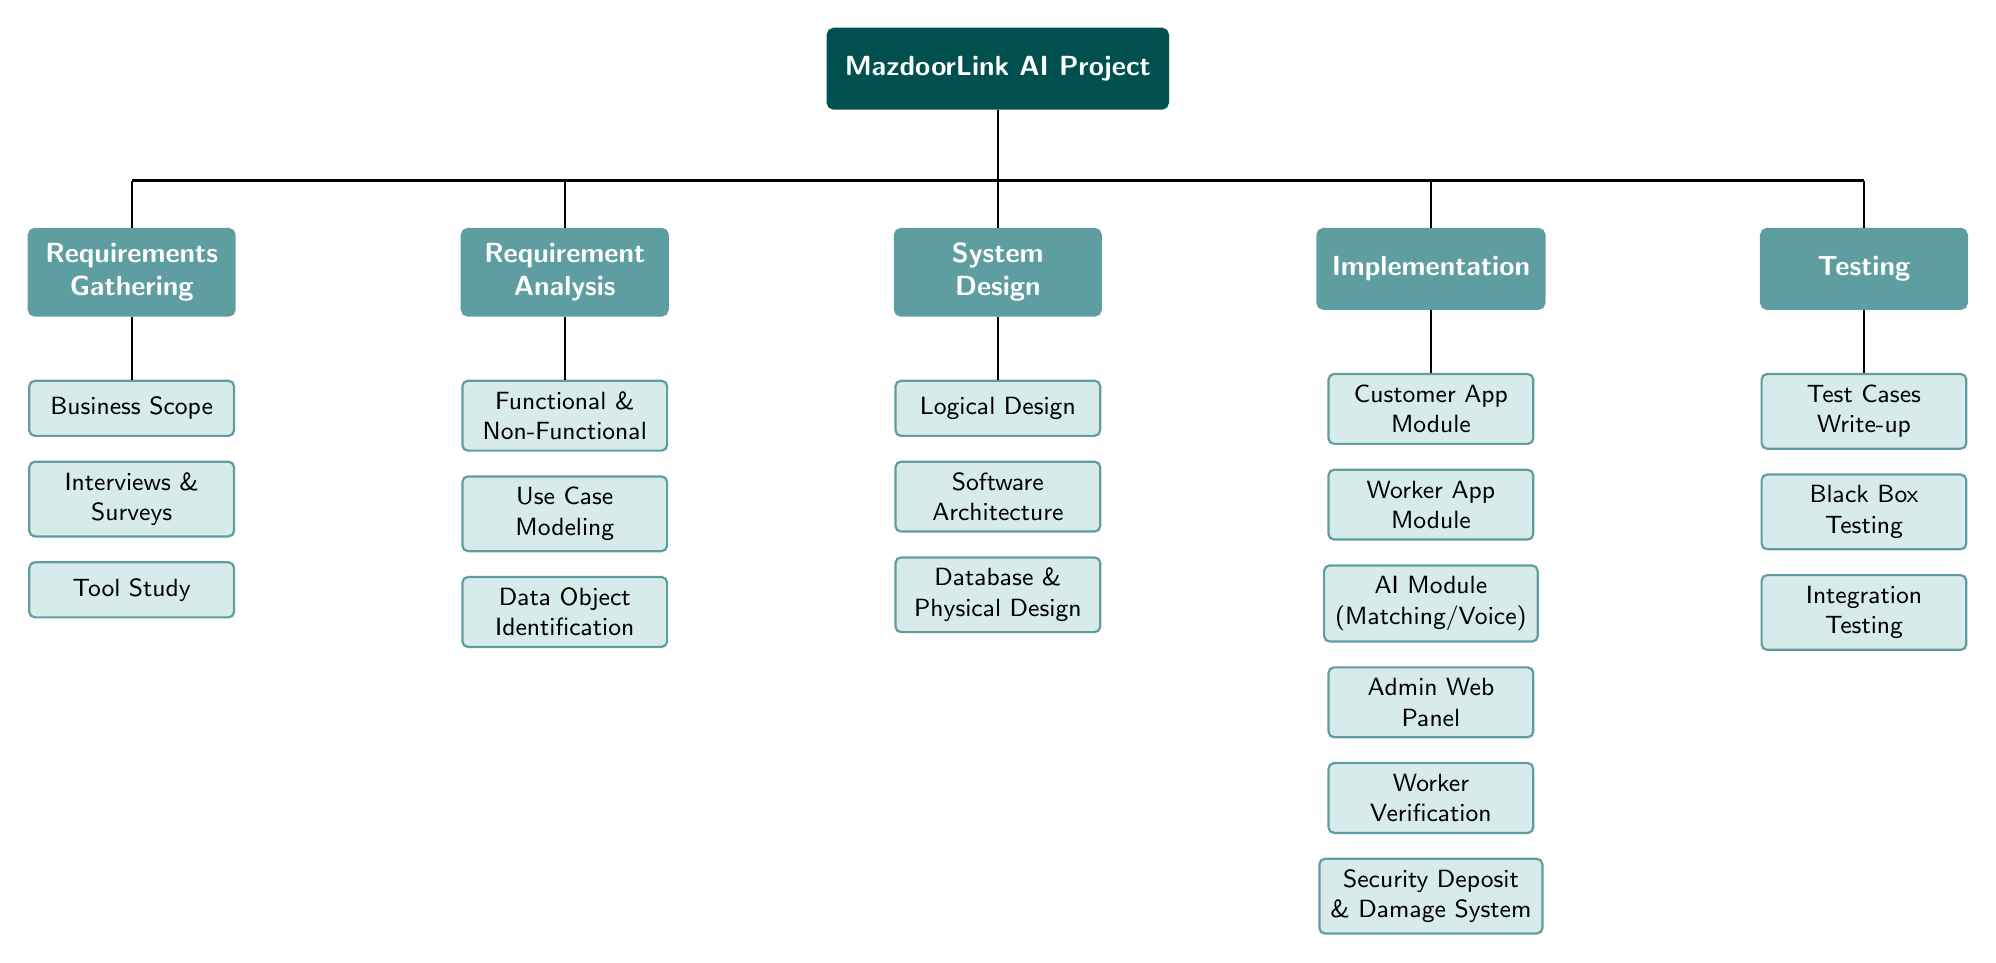
\begin{tikzpicture}[
        font=\sffamily\small,
        root/.style={
            rectangle, rounded corners=2pt, draw=wbsRoot, very thick,
            fill=wbsRoot, text=white, font=\sffamily\bfseries,
            minimum width=3cm, minimum height=1cm, align=center, inner sep=6pt
        },
        phase/.style={
            rectangle, rounded corners=2pt, draw=wbsPhase, very thick,
            fill=wbsPhase, text=white, font=\sffamily\bfseries,
            minimum width=2.6cm, minimum height=1cm, align=center, inner sep=5pt
        },
        task/.style={
            rectangle, rounded corners=2pt, draw=wbsPhase, thick,
            fill=wbsTask, font=\sffamily\small,
            minimum width=2.6cm, minimum height=0.7cm, align=center, inner sep=4pt
        },
        line/.style={draw=black, thick}
    ]

    % ROOT NODE
    \node[root] (root) at (0, 0) {MazdoorLink AI Project};

    % PHASE HEADERS (positioned in a row below root)
    \node[phase, below=1.5cm of root, xshift=-11cm] (p1) {Requirements\\Gathering};
    \node[phase, below=1.5cm of root, xshift=-5.5cm] (p2) {Requirement\\Analysis};
    \node[phase, below=1.5cm of root, xshift=0cm]    (p3) {System\\Design};
    \node[phase, below=1.5cm of root, xshift=5.5cm]  (p4) {Implementation};
    \node[phase, below=1.5cm of root, xshift=11cm]   (p5) {Testing};

    % CONNECT ROOT TO PHASES
    \draw[line] (root.south) |- ([yshift=0.6cm]p1.north);
    \draw[line] (root.south) |- ([yshift=0.6cm]p2.north);
    \draw[line] (root.south) |- ([yshift=0.6cm]p3.north);
    \draw[line] (root.south) |- ([yshift=0.6cm]p4.north);
    \draw[line] (root.south) |- ([yshift=0.6cm]p5.north);

    \draw[line] (p1.north) -- ++(0, 0.6);
    \draw[line] (p2.north) -- ++(0, 0.6);
    \draw[line] (p3.north) -- ++(0, 0.6);
    \draw[line] (p4.north) -- ++(0, 0.6);
    \draw[line] (p5.north) -- ++(0, 0.6);

    % PHASE 1: Requirements Gathering
    \node[task, below=0.8cm of p1] (p1t1) {Business Scope};
    \node[task, below=0.3cm of p1t1] (p1t2) {Interviews \&\\Surveys};
    \node[task, below=0.3cm of p1t2] (p1t3) {Tool Study};

    % PHASE 2: Requirement Analysis
    \node[task, below=0.8cm of p2] (p2t1) {Functional \&\\Non-Functional};
    \node[task, below=0.3cm of p2t1] (p2t2) {Use Case\\Modeling};
    \node[task, below=0.3cm of p2t2] (p2t3) {Data Object\\Identification};

    % PHASE 3: System Design
    \node[task, below=0.8cm of p3] (p3t1) {Logical Design};
    \node[task, below=0.3cm of p3t1] (p3t2) {Software\\Architecture};
    \node[task, below=0.3cm of p3t2] (p3t3) {Database \&\\Physical Design};

    % PHASE 4: Implementation
    \node[task, below=0.8cm of p4] (p4t1) {Customer App\\Module};
    \node[task, below=0.3cm of p4t1] (p4t2) {Worker App\\Module};
    \node[task, below=0.3cm of p4t2] (p4t3) {AI Module\\(Matching/Voice)};
    \node[task, below=0.3cm of p4t3] (p4t4) {Admin Web\\Panel};
    \node[task, below=0.3cm of p4t4] (p4t5) {Worker\\Verification};
    \node[task, below=0.3cm of p4t5] (p4t6) {Security Deposit\\\& Damage System};

    % PHASE 5: Testing
    \node[task, below=0.8cm of p5] (p5t1) {Test Cases\\Write-up};
    \node[task, below=0.3cm of p5t1] (p5t2) {Black Box\\Testing};
    \node[task, below=0.3cm of p5t2] (p5t3) {Integration\\Testing};

    % VERTICAL CONNECTORS (Phase to Tasks)
    \draw[line] (p1.south) -- (p1t3.south |- p1t1.north);
    \draw[line] (p2.south) -- (p2t3.south |- p2t1.north);
    \draw[line] (p3.south) -- (p3t3.south |- p3t1.north);
    \draw[line] (p4.south) -- (p4t6.south |- p4t1.north);
    \draw[line] (p5.south) -- (p5t3.south |- p5t1.north);

    \end{tikzpicture}
    }
    \caption{Project Work Breakdown Structure}
    \label{fig:wbs}
\end{figure}

Table \ref{tab:wbs} provides a detailed description of the work breakdown with the responsible team members for each task.

\begin{table}[!htbp]
    \centering
    \caption{Work Breakdown -- Task Assignment}
    \label{tab:wbs}
    \vspace{0.2cm}
    \begin{tabular}{cp{7cm}l}
        \toprule
        \textbf{Sr.} & \textbf{Task} & \textbf{Responsible Member(s)} \\
        \midrule
        1 & Requirements Gathering & Bilal, Hanzala, Wasif \\
        2 & Market Research \& Business Scope Analysis & Bilal \\
        3 & Stakeholder Interviews \& Surveys & Hanzala \\
        4 & Relevant Tool \& Technology Study & Wasif \\
        5 & Functional \& Non-Functional Requirements & Bilal, Hanzala \\
        6 & Use Case Modeling & Hanzala \\
        7 & Data Object Identification & Bilal \\
        8 & Logical Design & Bilal \\
        9 & Software Architecture & Wasif \\
        10 & Database \& Physical Design & Hanzala \\
        11 & Customer Mobile Application Module & Bilal \\
        12 & Worker Mobile Application Module & Hanzala \\
        13 & AI Module (Job Matching, Voice, Translation) & Wasif \\
        14 & Admin Interface Development & Bilal, Wasif \\
        15 & Worker Verification \& Security Deposit Module & Hanzala \\
        16 & Damage Reporting System & Bilal, Hanzala \\
        17 & Scheduled Bookings \& Time Tracker & Wasif \\
        18 & Service Photos \& Packages Feature & Hanzala \\
        19 & Test Cases Write-up & Hanzala \\
        20 & Black Box / Integration Testing & Wasif \\
        21 & Documentation & Bilal, Hanzala, Wasif \\
        \bottomrule
    \end{tabular}
\end{table}

\section{Project Timeline}

The proposed project timeline is aligned with the official FYP Calendar -- Spring 2026 issued by the Department of Computer Science, Capital University of Science and Technology. The project work formally commences after the Proposal Defense scheduled on 31st March 2026 (Tuesday). The timeline spans from April 2026 to December 2026, covering the complete development life cycle across the defined academic milestones.

The Gantt chart in Figure \ref{fig:gantt} illustrates the project schedule with task assignments mapped to the official FYP deadlines.

% ==========================================
% GANTT CHART
% ==========================================
\begin{figure}[!htbp]
    \centering
    \resizebox{\textwidth}{!}{
    \begin{ganttchart}[
        hgrid,
        vgrid,
        x unit=0.45cm,
        y unit title=0.5cm,
        y unit chart=0.6cm,
        title label font=\bfseries\footnotesize,
        bar label font=\scriptsize,
        group label font=\scriptsize\bfseries,
        milestone label font=\scriptsize\itshape,
        bar/.append style={fill=blue!30},
        group/.append style={draw=black, fill=gray!25},
        milestone/.append style={fill=red},
    ]{1}{36}

    % Month Titles
    \gantttitle{Apr}{4}
    \gantttitle{May}{4}
    \gantttitle{Jun}{4}
    \gantttitle{Jul}{4}
    \gantttitle{Aug}{4}
    \gantttitle{Sep}{4}
    \gantttitle{Oct}{4}
    \gantttitle{Nov}{4}
    \gantttitle{Dec}{4} \\

    % Phase 1: System & Database Design
    \ganttgroup{System \& Database Design}{1}{6} \\
    \ganttbar{Logical \& Architecture Design}{1}{4} \\
    \ganttbar{Database Schema \& UI/UX Design}{3}{6} \\

    % Phase 2: Core Module Implementation
    \ganttgroup{Core Module Implementation}{5}{26} \\
    \ganttbar{Auth \& Customer Mobile App}{5}{12} \\
    \ganttbar{Worker Mobile App \& Voice Module}{8}{16} \\
    \ganttbar{AI Job Matching \& Translation}{12}{20} \\
    \ganttbar{Chat System \& Communication}{16}{22} \\
    \ganttbar{Worker Verification \& Security Deposit}{18}{24} \\
    \ganttbar{Admin Interface \& Damage Reporting}{20}{28} \\

    % Phase 3: Integration & Testing
    \ganttgroup{Integration \& Testing}{25}{32} \\
    \ganttbar{API Integration \& Unit Testing}{25}{30} \\
    \ganttbar{Integration \& Acceptance Testing}{29}{32} \\

    % Phase 4: Documentation & Deployment
    \ganttgroup{Documentation \& Deployment}{31}{36} \\
    \ganttbar{Documentation \& Report Submission}{31}{34} \\
    \ganttbar{Deployment \& Presentation}{33}{36} \\

    % Milestones
    \ganttmilestone{Proposal Defense}{1} \\
    \ganttmilestone{Mid Report \& Exam}{14} \\
    \ganttmilestone{Final Report to REQRC}{24} \\
    \ganttmilestone{Final Report Submission}{29} \\
    \ganttmilestone{Final Exam}{35}

    \end{ganttchart}
    }
    \caption{Project Timeline -- April 2026 to December 2026}
    \label{fig:gantt}
\end{figure}

\newpage
% ==========================================
% BIBLIOGRAPHY
% ==========================================
\renewcommand\bibname{Bibliography}
\begin{thebibliography}{99}

\bibitem{ilo}
International Labour Organization, ``Women and Men in the Informal Economy: A Statistical Update,'' ILO Geneva, 3rd Edition, 2022.

\bibitem{pbs}
Pakistan Bureau of Statistics, ``Labour Force Survey 2022--2023 -- Annual Report,'' Government of Pakistan, 2023.

\bibitem{ahmed2021}
S.~Ahmed, M.~Hassan, and A.~Khan, ``Digital Divide and Technology Adoption Barriers among Blue-Collar Workers in South Asia: A Systematic Review,'' \textit{Journal of Information Technology for Development}, vol.~27, no.~4, pp.~512--530, 2021.

\bibitem{karsaaz}
Karsaaz, ``Karsaaz -- Home Services On Demand,'' [Online]. Available: \url{https://karsaaz.app/}. [Accessed: 10-Apr-2025].

\bibitem{kamkaaj}
Kam Kaaj, ``Kam Kaaj -- Home Services Platform,'' [Online]. Available: \url{https://kamkaaj.com/}. [Accessed: 10-Apr-2025].

\bibitem{homeservices}
HomeServices.pk, ``HomeServices.pk -- Find Home Service Providers in Pakistan,'' [Online]. Available: \url{https://homeservices.pk/}. [Accessed: 10-Apr-2025].

\bibitem{taskbid}
TaskBid, ``TaskBid -- Task-Based Hiring Platform,'' [Online]. Available: \url{https://taskbid.com/}. [Accessed: 10-Apr-2025].

\bibitem{worldbank}
World Bank Group, ``The Gig Economy in Developing Countries: Opportunities and Challenges,'' World Bank Policy Research Working Paper, 2023.

\bibitem{google_speech}
Google Cloud, ``Cloud Speech-to-Text API Documentation,'' [Online]. Available: \url{https://cloud.google.com/speech-to-text}. [Accessed: 10-Apr-2025].

\bibitem{google_translation}
Google Cloud, ``Cloud Translation API Documentation,'' [Online]. Available: \url{https://cloud.google.com/translate}. [Accessed: 10-Apr-2025].

\end{thebibliography}

\end{document}